\documentclass[10pt,twocolumn,letterpaper]{article}

\usepackage{cvpr}
\usepackage{times}
\usepackage{epsfig}
\usepackage{graphicx}
\usepackage{amsmath}
\usepackage{amssymb}

% Include other packages here, before hyperref.

% If you comment hyperref and then uncomment it, you should delete
% egpaper.aux before re-running latex.  (Or just hit 'q' on the first latex
% run, let it finish, and you should be clear).
\usepackage[pagebackref=true,breaklinks=true,letterpaper=true,colorlinks,bookmarks=false]{hyperref}

% \cvprfinalcopy % *** Uncomment this line for the final submission

\def\cvprPaperID{****} % *** Enter the CVPR Paper ID here
\def\httilde{\mbox{\tt\raisebox{-.5ex}{\symbol{126}}}}

% Pages are numbered in submission mode, and unnumbered in camera-ready
\ifcvprfinal\pagestyle{empty}\fi
\begin{document}

%%%%%%%%% TITLE
\title{Visual Census Using Cars}

\author{First Author\\
Institution1\\
Institution1 address\\
{\tt\small firstauthor@i1.org}
% For a paper whose authors are all at the same institution,
% omit the following lines up until the closing ``}''.
% Additional authors and addresses can be added with ``\and'',
% just like the second author.
% To save space, use either the email address or home page, not both
\and
Second Author\\
Institution2\\
First line of institution2 address\\
{\tt\small secondauthor@i2.org}
}

\maketitle
%\thispagestyle{empty}

%%%%%%%%% ABSTRACT
\begin{abstract}
Detecting a large number of BMWs in images informs us that those images may be of a wealthy area. Conversely, knowing that our images were obtained from a wealthy neighborhood increases the likelihood of detecting expensive cars. We explore this relationship between demographic factors and fine-grained classes by performing large scale detection of over 2600 car classes and conducting a social analysis of unprecedented scale in computer vision. Using 45 million images from 200 of the biggest cities in the United States, we predict demographic factors such as neighborhood wealth, education levels and show that our results correlate well with census data. To facilitate our work, we have collected the largest and most challenging fine-grained dataset reported to date consisting of over 2500 classes of cars comprised of images from google street view and other web sources and classified by car experts to account for even the most subtle of visual differences. We hope our work ushers in a new research area fusing fine-grained object detection and societal analysis.
\end{abstract}

\section{Introduction}
\begin{figure}[t]
\begin{center}
   \includegraphics[width=1\linewidth]{img/pull.jpg}
\end{center}
   \caption{Cars on the street provide information about people and their neighborhoods. Without location information, we can guess that images from the first column are from wealthy areas where as those from the second column are from poorer neighborhoods.}
\label{fig:pull}
\end{figure}

%%%%%%%%% BODY TEXT
\begin{figure*}[t]
\begin{center}
   \includegraphics[width=1\linewidth]{img/dataset_figure.jpg}
\end{center}
   \caption{Left: examples of cars from craigslist, cars.com and edmunds.com, Right: examples of cars from streetview images. Cars from streetview images are blurred and occluded.}
\label{fig:dataset1}
\end{figure*}
The artifacts with which we choose to surround ourselves tell us not only about ourselves but also about the society in which we live. In the 21st century, some of the most relevant objects defining people and their lifestyles are houses, clothes and cars. From a single picture such as fig.~\ref{fig:pull}a of an individual with their car, we can guess that the person is rich because they own a tesla, and that they probably care about the environment. Similarly, it is evident that figs.~\ref{fig:pull} b and c are of poorer neighborhoods where as figs.~\ref{fig:pull}1 and b are that of wealthy ones. Traditionally, the most prevalent method for gathering such personal and demographic information is through surveys such as census and American community survey (ACS) projects. However, the emergence of big and diverse sets of data generated by people has enabled computer scientists and computational sociologists to gain interesting insights by analyzing massive user texts and social networks~\cite{jure}~\cite{nlp_people}. For example, recent work from~\cite{ngrams} analyzed \(\sim 1\)M books and presented results related to the evolution of the english language as well as various cultural phenomena.

On the computer vision side, a few pioneering works by Torralba etal, Berg etal, and Hedalgo etal have recently started to apply visual scene analysis techniques to infer characteristics of neighborhoods and cities~\cite{antonio}~\cite{mcdonalds}~\cite{mit_cvpr}~\cite{tamara}.In this work, we are also interested in using images to understand cities, neighborhoods and the demographic makeup of their inhabitants. However, instead of using global image statistics, we achieve this goal by detecting and classifying cars on the street. 95\% of American households own cars~\cite{car_stats}, and as seen in fig.~\ref{fig:pull} cars give a lot of information about individuals as well as neighborhoods.

Our contributions are two-fold. First, we offer a fine-grained car dataset of unprecedented scale. It has 2657 car classes consisting of nearly all car types produced in the world after 1990: with a total of \(\sim 700\)k images from websites such as edmunds.com, cars.com, craigslist.com and street view (fig.~\ref{fig:dataset1}). Our testing dataset for social analysis consists of more than 45 million google street view images from 200 of the largest American cities and 2519 zip codes where an average of \(\sim\)18k images is collected for each zip code.

Second, our paper offers a suite of interesting social analysis of American people and cities using a large scale fine-grained object detection system. This work is only possible because of the tremendous progress in object recognition: particularly object detection and fine-grained object recognition. We use DPM~\cite{dpm}~\cite{dpm_web} to detect cars due to scalability concerns and train a CNN~\cite{alexnet} to classify them into one of 2567 classes. Using the result of our detections, we are able to offer insights into a number of very interesting questions related to our lives, communities and cities. Section~\ref{sec:social} shows a series of analyses about how the types of cars we drive relate to our level of education, wealth and the neighborhoods and cities we live in and section~\ref{sec:prior} presents preliminary results in exploring the use of demographic information to improve gine-grained car classification.



%------------------------------------------------------------------------
\section{Related Work}
\textbf{City analysis via image features}. There has been recent interest in using images to characterize cities~\cite{mit_plos_1}~\cite{tamara}~\cite{paris}~\cite{antonio}~\cite{mit_cvpr}~\cite{mcdonalds}. ~\cite{mit_plos_1} created scores for perceptions of wealth, safety and uniqueness by asking people to rate images from 3 cities on a scale of 1\textendash10 and ~\cite{mit_cvpr}~\cite{tamara} predicted these scores using various global image features such as GIST and CNN. In another line of work analyzing cities, ~\cite{antonio} perform city identity recognition after representing each city with higher level attributes. ~\cite{paris} identify unique qualities of cities such as Paris and Prague and~\cite{mcdonalds} shows that given an image of a particular city location, it is possible to predict the most likely direction for the location of a McDonalds. While our work also shares the motive of city analysis through imagery, it differs in that we use fine-grained object recognition to achieve this goal. As shown in section~\ref{sec:social}, this allows us to perform much more extensive social and demographic analysis through imagery and also easily extend our analysis to many other cities without the need for additional labeling.\newline\newline
\textbf{Fine-grained object recognition}. Fine-grained object recognition is a difficult problem due to the high visual similarity between classes. Nevertheless, recent works such as ~\cite{ning}~\cite{cars} show impressive results by using part annotated datasets such as ~\cite{birds}~\cite{dogs}~\cite{cars} and augmenting state of the art object detection algorithms such as RCNN~\cite{rcnn}. However, it is difficult to evaluate fine-grained classification accuracy since there are no fine-grained datasets that match object classification datasets like imagenet~\cite{imagenet} in the number of classes or images. Recent works such as~\cite{birdsnap} have introduced larger scale fine-grained datasets and ~\cite{nyc3d} has introduced a 3D car dataset annotated with metadata such as location information. We introduce a geotagged car dataset with unprecedented scale in both the number of classes and images.\newline\newline
\textbf{Using GPS data to improve classification}. Although an increasing number of images that we interact with daily are associated with GPS tags, there are very few computer vision algorithms that take advantage of location based metadata. However, recent works such as~\cite{amir} use location information to assist in detecting objects such as trash cans and street lamps,~\cite{birdsnap} learns a spatio-temporal prior to improve bird classification and~\cite{nyc3d} uses some location information such as elevation to assist in car classification. 

%------------------------------------------------------------------------
%\begin{figure} [t]
%\begin{center}
%\includegraphics[width=0.8\linewidth]{img/car_hierarchy.jpg}
%\end{center}
%\caption {Car class hierarchy. Classes are usually more visually similar when we travel down the tree.}
%\label{fig:hierarchy}
%\end{figure}

\begin{figure*} [t]
\begin{center}
\raisebox{0.5\height}{
  \includegraphics[width=0.25\linewidth]{img/car_hierarchy.jpg}
}
\includegraphics[width=0.32\linewidth]{img/web.jpg}
\includegraphics[width=0.32\linewidth]{img/street.jpg}
\end{center}
\caption {Left: A hierarchy of car classes where images become more difficult to distinguish while travelling down the tree.The leaves (e.g. class 1 and class 2) are the fine-grained classes. Center: Class image distribution for web images. We have the most number of images for 2001-2003 Hyundai Elatra sedan glx and the least for 1990-1992 Audi 80 sedan base. Right: class image distribution for street view images.}
\label{fig:img_dist}
\end{figure*}

\section{Cars and Cities Dataset}
\label{sec:data}
\begin{figure}[t]
\begin{center}
   \includegraphics[width=0.45\linewidth]{img/loc_prior.png}
   \includegraphics[width=0.45\linewidth]{img/bbox_heat.png}
\end{center}
   \caption{Left: Location/scale heatmap of streetview bounding boxes with red indicating larger sizes and blue smaller ones. Each point indicates the size of a bounding box centered at that point in a street view image.}
   \caption{Right: Heatmap of streetview bounding box locations. Most cars are located in a line slightly below the center of the image.}
\label{fig:loc-heat}
\end{figure}

\begin{table}
\begin{center}
\begin{tabular}{|l|c|c|r|}
\hline
\textbf{Attribute} & \textbf{Train} & \textbf{Val} & \textbf{Test} \\
\hline\hline
No. streetview bboxes & 34,712 & 6,915 &27,865\\
No. web bboxes & 313,099 & - &-\\
No. web images & 313,099 & - &-\\
No. streetview images & 199,666 & 39,933 &159,732\\
No. Total images &512,765&39,933&159,732\\
No. classes & 2657 & - & -\\
No. car types & 18017 & - & -\\
\hline
\end{tabular}
\end{center}
\caption{Street view data statistics}
\label{table:data}
\end{table}
We first collected 45 million images from 8 million GPS points by sampling the roads of 200 of the biggest US cities every 25m. For each GPS coordinate we gathered street view images at 0, 60, 120, 180, 240, 300 degree rotations. In order to train a fine-grained car classifier to detect and classify the cars in our images, we created the largest ever reported fine-grained dataset of cars consisting of all the cars listed on edmunds.com (all cars manufactured after 1990). To assemble our car dataset we obtained images of all cars in edmunds.com (\(\sim18k\)cars) and grouped the cars into visually indistinguishable classes using a series of amazon mechanical turk tasks. After creating a class list, we collected additional images of cars from cars.com as well as craigslist and used AMT to annotate them with bounding boxes. Finally, we hired car experts to label \(\sim 70\)k bounding boxes of cars from the street view images with fine-grained lables. We also labeled cars from craigslist and cars.com by parsing the car posting titles. 

Table~\ref{table:data} summarizes the statistics of our dataset and fig.~\ref{fig:dataset1}a shows some examples. We can see that cars from street view images are generally occluded and blurry where as those from other web sources have higher resolution. As seen in fig.~\ref{fig:loc-heat}, the street view bounding boxes are distributed in a line around the center of the image and bounding boxes near the center also occupy a larger space. Fig.~\ref{fig:img_dist}a, shows a hierarchy of classes in our dataset where classes become increasingly visually indistinguishable while traveling down the tree. As the figure shows, the difference between leaf classes such as class 1 and class 2 is extremely subtle. Finally fig.~\ref{fig:img_dist}a and b show the distribution of street view and web images for different classes. 

\section{Detecting and classifying cars}
\label{sec:detection}
Although RCNN based fine-grained detection algorithms have reported state of the art results, ~\cite{rcnn}~\cite{ning}, its computational and memory requirements make it impractical for use in a large scale detection setting such as ours. In addition to memory requirements, detecting cars in our images would take \(\sim\)20s per image using a machine with a single GPU. Thus our pipeline, instead, consists of using DPM~\cite{dpm} to detect cars and a CNN ~\cite{alexnet} to classify them. We present details in the sections below.

\subsection{Car Detection}
Inorder to evaluate accuracy/speed trade off, we trained DPMS with different numbers of components and parts and used the model with the best tradeoff for detection. Our final algorithm employs a single component 8 part DPM and achieves an AP of 64.2\% while taking 5 secs per image. As a point of comparison, the highest AP (68.7\%) was achieved with a 5 component 8 part DPM which takes \(\sim\)22 secs per image. Detailed plots and timing measurements of other DPMs we have trained are discussed in our supplementary material.


\begin{table}
\begin{center}
\begin{tabular}{|l|c|}
\hline
\textbf{Attribute} & \textbf{Acc\%} \\
\hline\hline
Make & 66.38 \\
Model & 51.83 \\
Submodel & 77.74 \\
%Year (5 bins) & X \\
Price (5 bins)& 61.61 \\
Domestic/Foreign & 87.71\\
Country & 84.21\\
\hline
\end{tabular}
\end{center}
\caption{Accuracy by car attribute}
\label{table:att-acc}
\end{table}

\begin{figure}[t]
\begin{center}
   %\includegraphics[width=1\linewidth]{img/price_confusion.png}
   \includegraphics[width=1\linewidth]{img/submodel_confusion.png}
\end{center}
   \caption{Confusion matrix for car submodel. As expected, the confusion is between similar types of submodels such as a sedan and coupe or an extended cab and a crew-cab.} 
\label{fig:confusion}
\end{figure}

\begin{figure} [t]
\begin{center}
\includegraphics[width=0.55\linewidth]{img/good_det.png}
\raisebox{-0.02\height}
 {
\includegraphics[width=0.34\linewidth]{img/cars.jpg}
 }
\end{center}
\caption {An example of our car detections and classifications. The red boxes are DPM bounding boxes that are not classified by our CNN and green boxes are boxes classifyied by the CNN. The two cars in the image are correctly classified to the classes shown on the right.}
\label{fig:dets}
\end{figure}

\subsection{Car Classification}
We use a standard CNN from ~\cite{alexnet} with ~\cite{caffe} to classify the DPM detections into one of 2657 fine-grained classes. Although our test set consists of street view images, as mentioned in sec.~\ref{sec:data} 61\% of our positive training images are composed of cars from other sources such as craigslist. Thus we add deformations such as blurring to these images during training to liken them to street view images. We give details of training the CNN in our supplementary material. At test time we take the top 10\% scoring DPM bounding boxes and classify them. This results in a 10x increase in speed but only a \(\sim\)2\% drop in AP as compared to using all the bounding boxes detected by DPM. We achieve an accuracy of 33.1\% on the true positive DPM bounding boxes and 31.27\% on the ground truth bounding boxes. Fig.~\ref{fig:good_dets} shows an example of our street view detections. The cars are detected and classified correctly even though blurriness and occlusions in street view images makes this a difficult task. Fig.~\ref{fig:confusion} shows a confusion matrix for submodel level classifications. It can be seen that most of the errors are between highly similar submodels such as sedan and coupe.   

\subsection{Analyzing Hierarchical Classification Accuracy}
Some types of classification mistakes are more costly than others for the task of social analysis. For example, an error misclassifying 2001 Honda Accord lx to 2001 Honda Accord dx is not significant. However, misclassifying a 2012 BMW 3-series to a 1996 Honda Accord,for example, would create large errors in an analysis measuring the realtionship between the average car price or age in a zip code and median household income. In order to gain more insight into the types of errors our classifier makes, we measure the accuracy of classifying different car attributes. Table~\ref{table:att-acc} lists accuracies by various car attributes such as those in fig.~\ref{fig:img_dist}a and others like car price, year etc\ldots We can see that the accuracy is much higher after aggregating by different attributes.  

 \section{Societal analysis}
\label{sec:social}
In this section, we present societal analysis results from all 200 cities as well as case studies from those with available ground truth data. We divide our analysis into different sections below.

\subsection{What cars on the street tell us about people}
\subsubsection{Sanity Check: Cars on the street correlate well with registred cars}
How do cars on the street relate to the cars that people drive? Specifically, can we learn about the registered cars in a zip code from our street view detections?
We downloaded vehicle census data from Massachusetts, which is the only state to release extensive vehicle registration data, and found an extremely high Pearson correlation coefficient of 0.9 (p \(\sim\)0) between the number of cars we detected per zip code and the number of cars that are registered. The high correlation was only obtained after aggregating cars at the zip code level which shows that most people in MA drive within their zip code. 
After establishing a high correlation between the number of cars we detect and the number of registered cars, we also measured the correlation between the make of the detected and registered cars per zip code. As we can see in fig.~\ref{fig:ma_corrs} there is a high correlation for most of the makes. Thus the cars we detect from street view images contain useful information about the types of cars driven by people in a particular zip code.

\begin{table}
\begin{center}
\begin{tabular}{|l|c|r|}
\hline
\textbf{Census Variable} & \textbf{Car Attribute} & \textbf{r}  \\
\hline\hline
Household income & No. 1990-1994 cars & -0.42 \\
Household income & No. 1995-1999 cars & -0.40 \\
Household income & No. 2000-2004 cars & 0.21 \\
Household income & No. 2005-2009 cars & 0.46 \\
Household income & \% foreign cars & 0.59 \\
Household income & \% German cars & 0.57 \\
Household income & \% Us cars & -0.59 \\
Household income & Avg. price & 0.49 \\
Education: highschool & Avg. price & -0.21 \\
Education: college & Avg. price & 0.32 \\
Education: graduate scl. & Avg. price & 0.39 \\
\hline
\end{tabular}
\end{center}
\caption{Pearson correlation coefficient between various census variables and detected car attributes. All p values are \(\sim\) 0.}
\label{table:car-census-corrs}
\end{table}

\begin{figure}[t]
\begin{center}
   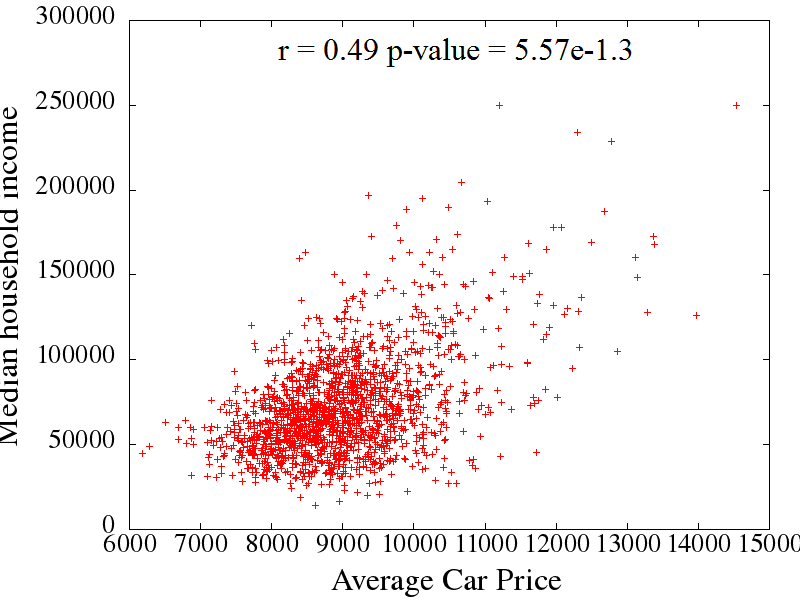
\includegraphics[width=0.9\linewidth]{img/averagePriceIncome.png}
\end{center}
   \caption {Scatter plot of median household income per zip code vs. average price of detected cars per zip code.}
\label{fig:price-income-corr}
\end{figure}

\begin{figure*} [t]
\begin{center}
\raisebox{-0.03\height}{
\includegraphics[width=0.3\linewidth]{img/boston_make_corr.png}
}
%\raisebox{0.3\height}{
  \includegraphics[width=0.3\linewidth]{img/boston_acura_corr.png}
%}
%\raisebox{0.3\height}{
\includegraphics[width=0.3\linewidth]{img/boston_bmw_corr.png}
%}
\end{center}
\caption {Left: Pearson correlation coefficient and p values between the number of detected and registered cars in Boston for each make. Center: scatter plot of detected cars per zip code vs. registered cars per zip code in Boston. Left: scatter plot of No. of detected Honda's per zip code vs. registered Honda's per zip code in Boston.}
\label{fig:ma_corrs}
\end{figure*}

\subsubsection{What do rich/poor people drive?}
We gathered zip code level as well as census tract level 2007-2012 American Community Survey data for the 200 cities in our dataset and analyzed how the census data relates to statistics from our detected cars. 

Table \ref{table:car-census-corrs} shows correlation values between various attributes of the detected cars and median household income as well as education level per zip code. Fig.~\ref{fig:price-income-corr} shows a plot of median household income vs. average car price in a zip code. As expected, there is a high correlation between median household income and the average car price per zip code (r=0.49, p \(\sim\) 0). Our results also indicate that rich people prefer to drive foreign, especially German, cars (r=0.59). What is perhaps surprising is that there is a very high negative correlation (r=-0.55, p \(\sim\) 0) between the percentage of American cars in a zip code and median household income. So poor people live in places with many American cars.

Poor people also live near very old cars where as rich people live near newer ones. As table \ref{table:car-census-corrs} shows, the correlation between median household income and the number of cars in 1990-1994 is very negative and increases to a high positive 0.59 for cars in the 2005-2009 range. Finally, a perhaps not surprising result is that poor people live near cars with low miles per gallon (MPG). This corroborates~\cite{cal-traffic-study} study showing that poor people are more exposed to car pollution than rich people.
 
\begin{figure*}[t]
\begin{center}
    \includegraphics[width=1\linewidth]{img/income_price.png}
    %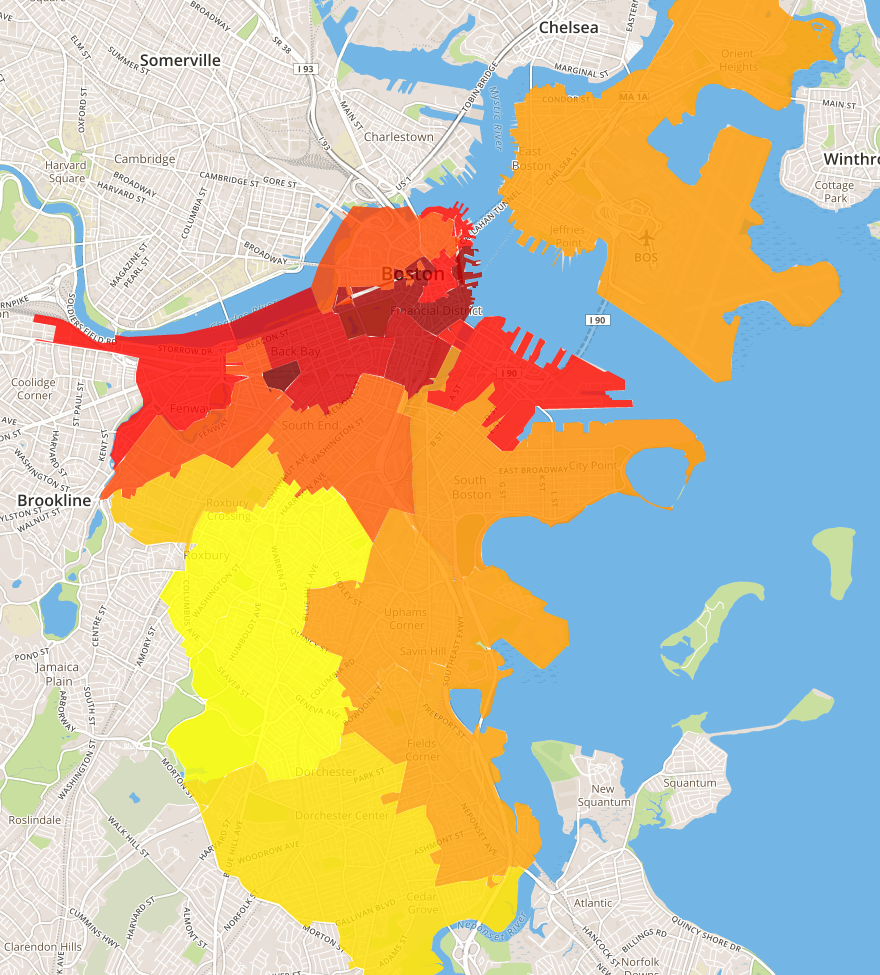
\includegraphics[width=0.45\linewidth]{img/price.png}
    %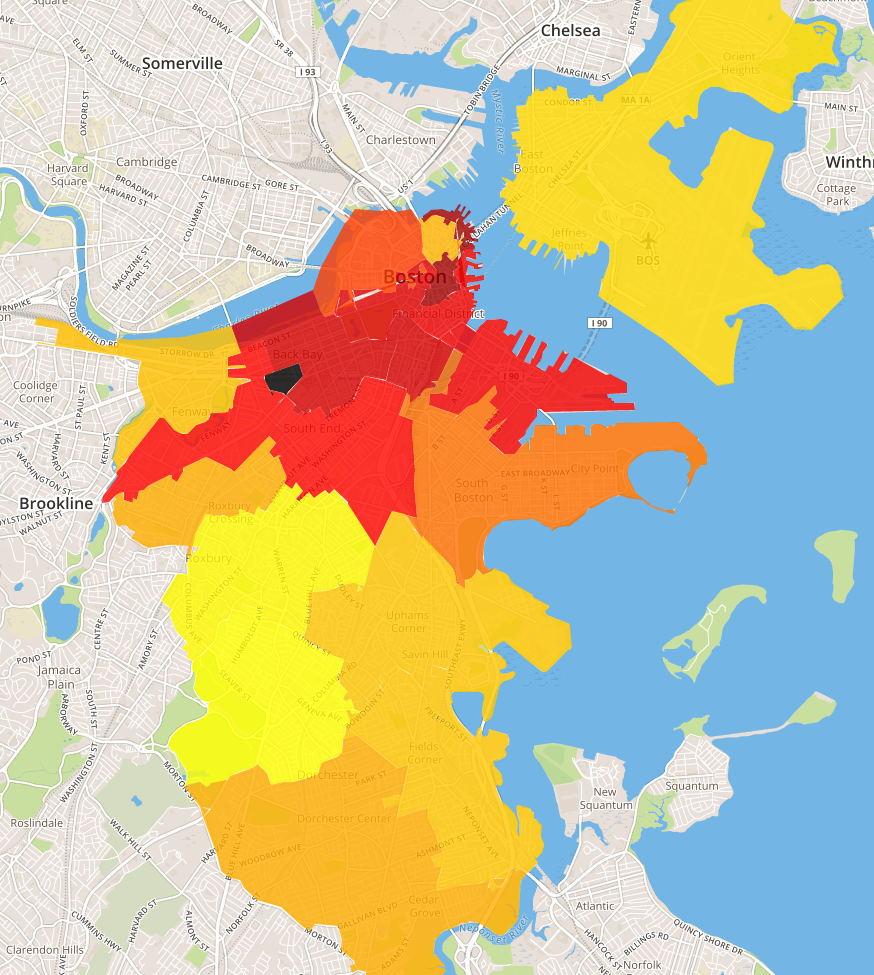
\includegraphics[width=0.45\linewidth]{img/income.png}
  %\raisebox{-.5\height}{
  % 
  %  \includegraphics[width=0.45\linewidth]{img/houston_income.png}
  %}
\end{center}
   \caption {Top left: Heat map of average car price in Boston, center: heat map of median household income in Boston. Bottom left: Heat map of average car price in Houston, center: heat map of median household income in Houston. Left example of street view images and car detections corresponding to zip codes with high and low incomes. Low income areas have many cheap cars where as high income areas have expensive ones.}
\label{fig:bos-sf-vis}
\end{figure*}

\subsubsection{How does education relate to cars on the street?}
As shown in \ref{table:car-census-corrs} there is a high negative correlation between the number of people with only a high school education and the average price of a car in a zip code. As expected, we also found a high correlation between the number of college educated people in a zip code and the average car price. What is perhaps surprising is that although there is a large increase in correlation coefficient from high school to college educated, the jump from college to graduate school is very low. Thus, there is a negligable difference in the price of cars driven by people who hold bachelors vs. graduate degrees.

\begin{figure}[t]
\begin{center}
  %\raisebox{-.02\height}
 %{
 %  \includegraphics[width=0.3\linewidth]{img/sf_density.png}
 %}
 %  \includegraphics[width=0.3\linewidth]{img/sf_mpg.png}
 %  \includegraphics[width=0.3\linewidth]{img/sf_air_cropped.png}
 %  \includegraphics[width=0.28\linewidth]{img/miami.png}
 %  \includegraphics[width=0.3\linewidth]{img/new_orleans.png}
 %  \includegraphics[width=0.26\linewidth]{img/portland.png}
    \includegraphics[width=1\linewidth]{img/mpg.png}
\end{center}
   \caption {A. Density of cars in San francisco inversely weighted by their expected miles per gallon (MPG), B. The inverse of weighted average of car MPG in San Francisco. The weights are the expected number of cars in a GPS point, C. Ground Truth for Air quality (measured in annual particulate matter) in San Francisco from~\cite{ground_air}.}
\label{fig:pollution}
\end{figure}

\subsection{What cars on the street tell us about neighborhoods}
\subsubsection{Which neighborhoods are wealthy/poor?}
Intuitively, seeing many expensive cars on the street indicate that we are in a rich neighborhood and vice versa. Figure \ref{fig:bos-sf-vis} A shows a heat map of the average price of detected cars within a zip code and median household income in a zip code for Boston and figure \ref{fig:bos-sf-vis} B shows the same visualization for Houston. We can see that in both cities, the average car price in a zip code is a very good predictor of wealthy/un-wealthy neighborhoods.


\subsubsection{Which neighborhoods have high car pollution?}
Can our street view detections tell us anything about which neighborhoods are affected by highly polluting cars? We plotted a heat map of the expected number of cars per sample inversely weighted by the expected MPG of that sample. We also map the inverse of the weighted average of car MPG where the weights are the expected number of cars. The first measure should give us a rough idea of the location of highly polluting neighborhoods: for the same density of cars, areas with high MPG result in lower numbers than those with low MPG. For different densities of cars, the relative magnitude of the measure depends on both the density of cars and how efficient they are. The second measure, on the other hand, visualizes areas with a high concentration of low MPG cars.

Fig.~\ref{fig:pollution}A shows the weighted density of cars in San Francisco and B shows the inverse weighted MPG. Although we could not find ground truth data of car pollution, Fig.~\ref{fig:pollution}C is a map of San Francisco air quality measuring annual average particulate matter concentration (MPG) from all sources~\cite{ground_air}. To our surprise, their map seems to agree with Fig.~\ref{fig:pollution}B in most cases.

\subsection{What cars on the street tell us about cities}
\subsubsection{Which cities are more segregated?}
Which cities show high clustering of similarly priced cars? Specifically, which cities have expensive cars clustered together with other expensive cars and cheap cars clustered with other cheap cars? Given the high correlation between median household income and average car price, the answer to this question should give us a good indication of the cities that are most and least segregated. Following the analysis of ~\cite{mit_plos_1} we use the Moran I statistic to measure spatial autocorrelation where a value of 1 indicates perfect clustering of similar values, -1 indicates perfect dispersion and 0 indicates a random spatial arrangement (neither clustering nor dispersion). Fig.~\ref{fig:moran-i} plots the highest and lowest scoring cities as well as well as a few others in between. We can see that Reno shows the highest clustering where as Dover shows the lowest.

\begin{figure}[t]
\begin{center}
    \includegraphics[width=0.9\linewidth]{img/moran.png}
\end{center}
   \caption {Moran I scores for car prices. The highest and lowest scoring cities are shown as well as 5 cities with scores in between. Reno exhibits the most amount of clustering by car price where as Dover exhibits very little clustering. The two maps for Boston and Dover show areas of high clustering where green indicates statistically significant clustering of expensive cars and red indicates statistically significant clustering of cheap cars.} 
\label{fig:moran-i}
\end{figure}

\subsubsection{Which cities are more patriotic?}
Which cities have the most number of domestic cars? As Fig.~\ref{fig:city_price}A shows the coastal cities have a high concentration of foreign made cars where as the midwest has a low concentration. This result agrees with ~\cite{foreign_domestic} who measured the ratio of American/foreign cars driven in the US. The city with the highest percentage of foreign cars was found to be San Francisco with 61\% of foreign cars where as Casper Wyoming had the least percentage (21\%).

\subsubsection{Which cities are wealthier?}
Which city has the most expensive cars on average? Fig.~\ref{fig:city_price}B maps the average car price for each city. The map shows that many of the east coast cities have expensive cars as well as some cities in the south such as Atlanta. We found the city with the most expensive cars to be New York with an expected price of \(\sim\)\$12k and the one with the least expensive cars to be El Paso (\(\sim\)\$7k). 

\begin{figure}[t]
\begin{center}
    \includegraphics[width=1\linewidth]{img/city_foreign_new.png}
    \includegraphics[width=1\linewidth]{img/foreign.png}
\end{center}
   \caption {Map of the percentage of foreign cars in each city. San Francisco has the highest percentage with (61\% and Casper the lowest with 21\%.} 
\label{fig:city_price}
\end{figure}

\begin{figure}[t]
\begin{center}
    \includegraphics[width=1\linewidth]{img/city_price_new.png}
\end{center}
   \caption {Map of the United States showing the expected car price in each city. New York has the highest expected car price where as El Paso has the lowest.}
\label{fig:city_price}
\end{figure}

\begin{table}
\begin{center}
\begin{tabular}{|l|c|r|}
\hline
\textbf{Attribute} & \textbf{Census Variable}& \textbf{Acc\%}\\
\hline\hline
Price & Median hh income & 31.60\\
Year  & Median hh income & 31.60\\
Make & No. ppl in management & 31.57\\
Submodel & Median hh income & 31.57\\
Domestic & No. ppl in managemenet & 31.54\\
Country & No. ppl in management & 31.54\\
\hline
\end{tabular}
\end{center}
\caption{Census variables resulting in the highest accuracy gain for each car attribute. Car price/year with median household income give the highest gain in accuracy.}
\label{table:prior-acc}
\end{table}

\section{Using social priors to improve classification}
\label{sec:prior}
This section explores the use of demographic census information as a prior to improve fine-grained detection and presents preliminary results run on our validation set. Intuitively, if a particular image was taken in a wealthy neighborhood, for example, one would expect the cars in that neighborhood to be expensive and viseversa. In order to use zip code level census variables as priors, we first calculated \(P(C|I,S)\) where \(C\) is the fine-grained class, \(I\) is an image and \(S\) \(\in\) \(\{\)\(S_{1}\)\ldots \(S_{n}\)\(\}\)is a particular zip code level census variable such as median household income. After applying Bayes' rule, assuming that the image and census data are conditionally independent given the class label, and applying Bayes' rule again we get:

\begin{equation}
P(C|I,S)\propto \frac{P(C|I)}{P(C)}P(C|S)
\label{eq:prior-eq}
\end{equation}

Where \(P(C|I)\) is the output of our CNN classifier. A naive way of using census variables such as the one above reduces accuracy by \(\sim\)5\% to ~26.1\%. This is not surprising given that we have over 2600 fine-grained classes, and many of them have similar attributes such as price. Thus, instead of using census variables directly as fine-grained class priors, we use them as priors for the car attributes. In order to incorporate these variables into our classification pipeline we can reformulate \(P(C|S)\) in equation~\ref{eq:prior-eq} as \(P(C|A)\)\(P(A|S)\) where \(A\) \(\in\) \(\{\)\(A_{1}\)\ldots\(A_{n}\)\(\}\) represents a car attribute such as price. After this modification, equation~\ref{eq:prior-eq} can be written as  

\begin{equation}
  P(C|I,S) \propto \frac{P(C|I)}{P(C)}P(C|A)P(A|S)
\end{equation}
We calculate \(P(C|I,S)\) for all car attributes and 30 different census variables, quantizing some car attributes and census variables such as car price and median household income into bins ranging from 2-20. Table~\ref{table:prior-acc} shows the highest accuracy numbers for various combinations of census variables and car attributes. It can be seen that using median household income and either car price or year give the highest accuracy gain. This result is to be expected since, as seen in section~\ref{sec:social}, there is a high correlation between median household income and car price and year. Although the accuracy gain at the fine-grained level is very slight (which is to be expected due to the large number of similar classes in our dataset). Our supplemental material discusses more extensive experiments and results in using census variables to improve our fine-grained classifications.

\section{Conclusion}
In conclusion, by analyzing car detections from 45 million images across 200 cities, we have shown that cars detected from street view images contain predictive information about our neighborhoods, cities and their demographic makeup. To facilitate this work, we have collected the largest and most challenging fine-grained dataset reported to date. For our future work we plan to perform more extensive social analysis\textemdash such as crime prediction and predicting changes in cities across time\textemdash using fine-grained detection. We also hope to further explore the use of demographic data to assist in fine-grained detection. 
{\small
\bibliographystyle{ieee}
\bibliography{egbib}
}

\end{document}

{\small
\bibliographystyle{ieee}
\bibliography{egbib}
}
\end{document}

 
